
\documentclass[12pt,oneside,reqno]{article}
%\documentclass[]{article}
\usepackage[margin=2cm]{geometry}
\usepackage[usenames]{color} %used for font color
\usepackage{bigints}
\usepackage{amssymb} %maths
\usepackage{amsmath} %maths
\usepackage{amsthm} %theorem environment
\usepackage{mathabx} %cartesian product environment
\usepackage{centernot} %to make not symbol centered
\usepackage[utf8]{inputenc} %useful to type directly diacritic characters
\usepackage{appendix}
\usepackage{apacite}
\bibliographystyle{apacite}
\usepackage [english]{babel}
\usepackage [autostyle, english = american]{csquotes}
\MakeOuterQuote{"} %to correct the quote symbol
%\usepackage{dirtytalk} %to make quotations in quotations
\usepackage{verbatim} %comment environment
\usepackage{enumerate}
\usepackage{sgame}
\usepackage{amsmath}
\usepackage{amsfonts}
\usepackage{amssymb}
\usepackage[framed,numbered,autolinebreaks,useliterate]{listings}
\usepackage{graphicx}
\graphicspath{ {images/} }
\usepackage{setspace} %spacing
\setlength{\parindent}{0pt}
\doublespacing

\theoremstyle{definition}
\newtheorem{definition}{Definition}[section]
\theoremstyle{definition}
\newtheorem{example}{Example}[section]
\theoremstyle{definition}
\newtheorem{lemma}{Lemma}[section]
\theoremstyle{definition}
\newtheorem{proposition}{Proposition}[section]
\theoremstyle{definition}
\newtheorem{claim}{Claim}[section]
\theoremstyle{definition}
\newtheorem{theorem}{Theorem}[section]
\theoremstyle{definition}
\newtheorem{axiom}{Axiom}[section]
\theoremstyle{definition}
\newtheorem{assumption}{Assumption}[section]
\newtheorem{remark}{Remark}[section]
\theoremstyle{definition}


%opening
\title{HW2 Report}
\author{Ece Teoman}

\begin{document}
	
	\maketitle
	\section*{}
	
	Here, I include the code and the output but the m.files and the diary can be found in the directory.
	
	\section{}

The resulting demands for the given parameterization are as follows:
\begin{lstlisting}

	D_A =

0.4223

D_B =

0.4223

D_0 =

0.1554

\end{lstlisting}


	\section{}

Given $q_A = q_B = 2$, solving for the Nash pricing equilibrium by using Broyden method results in the following:

\begin{lstlisting}

sol_broyden =

1.5989    1.5989


Broyden_runtime =

0.0284


\end{lstlisting}

	\section{}

Under the same parameter values, now using Gauss-Seidel method to solve for the pricing equilibrium results in the following:

\begin{lstlisting}

solution_Gauss_Seidel =

1.5989
1.5989


Gauss_Seidel_runtime =

0.3158


\end{lstlisting}

In this case, Broyden was faster than Gauss-Seidel.

	\section{}

Solving for the equilibrium using the given update rule results in:

\begin{lstlisting}
solution_update =

1.5989
1.5989

update_runtime =

0.0048

\end{lstlisting}

It converges and this method is the fastest so far. 
\newpage

	\section{}

Given the parameters, the resulting pricing equilibrium, by using Gauss-Seidel method is:

\begin{lstlisting}
	p_a =
	
	Columns 1 through 12
	
	1.8671    1.8465    1.8239    1.7995    1.7735    1.7461    1.7176    1.6883    1.6586    1.6287    *1.5989*    1.5697
	
	Columns 13 through 16
	
	1.5411    1.5134    1.4867    1.4612
	
	p_b =
	
	Columns 1 through 12
	
	1.1481    1.1743    1.2041    1.2378    1.2757    1.3179    1.3646    1.4160    1.4721    1.5331    *1.5989*    1.6697
	
	Columns 13 through 16
	
	1.7453    1.8257    1.9109    2.0008
	
\end{lstlisting}

So the equilibrium prices are the same as in the previous parts. The resulting graph is as follows:

\begin{figure}[!h]
	\centering
	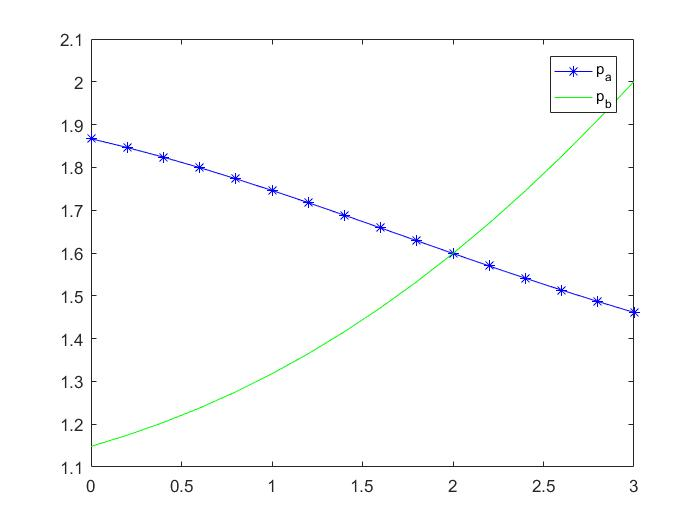
\includegraphics[width=0.7\linewidth]{q5}
	\caption{}
	\label{}
\end{figure}


\newpage\

\section{MATLAB codes}

Here are the functions and the rest of the code I've written to get the answers above:

\subsection{Functions}

\lstinputlisting{demand.m}
\lstinputlisting{foc.m}
\lstinputlisting{onestep.m}
\lstinputlisting{price_update.m}

\subsection{Main}
\lstinputlisting{main.m}

\end{document}